%-------------------------------------------------------------------------------
\Section{Muon-based Accelerators} \par
Muons ($\mu$) were first discovered experimentally in 1947 by Powell \emph{et al.} \cite{griffithspp} who were looking for the Yukawa meson.
It is now known that muons fit into a particle group called leptons, and fit into the standard model (along with other fundamental particles) as shown in Figure 1.

\begin{figure}[h!]
\label{fig:standardmodel}
\centering
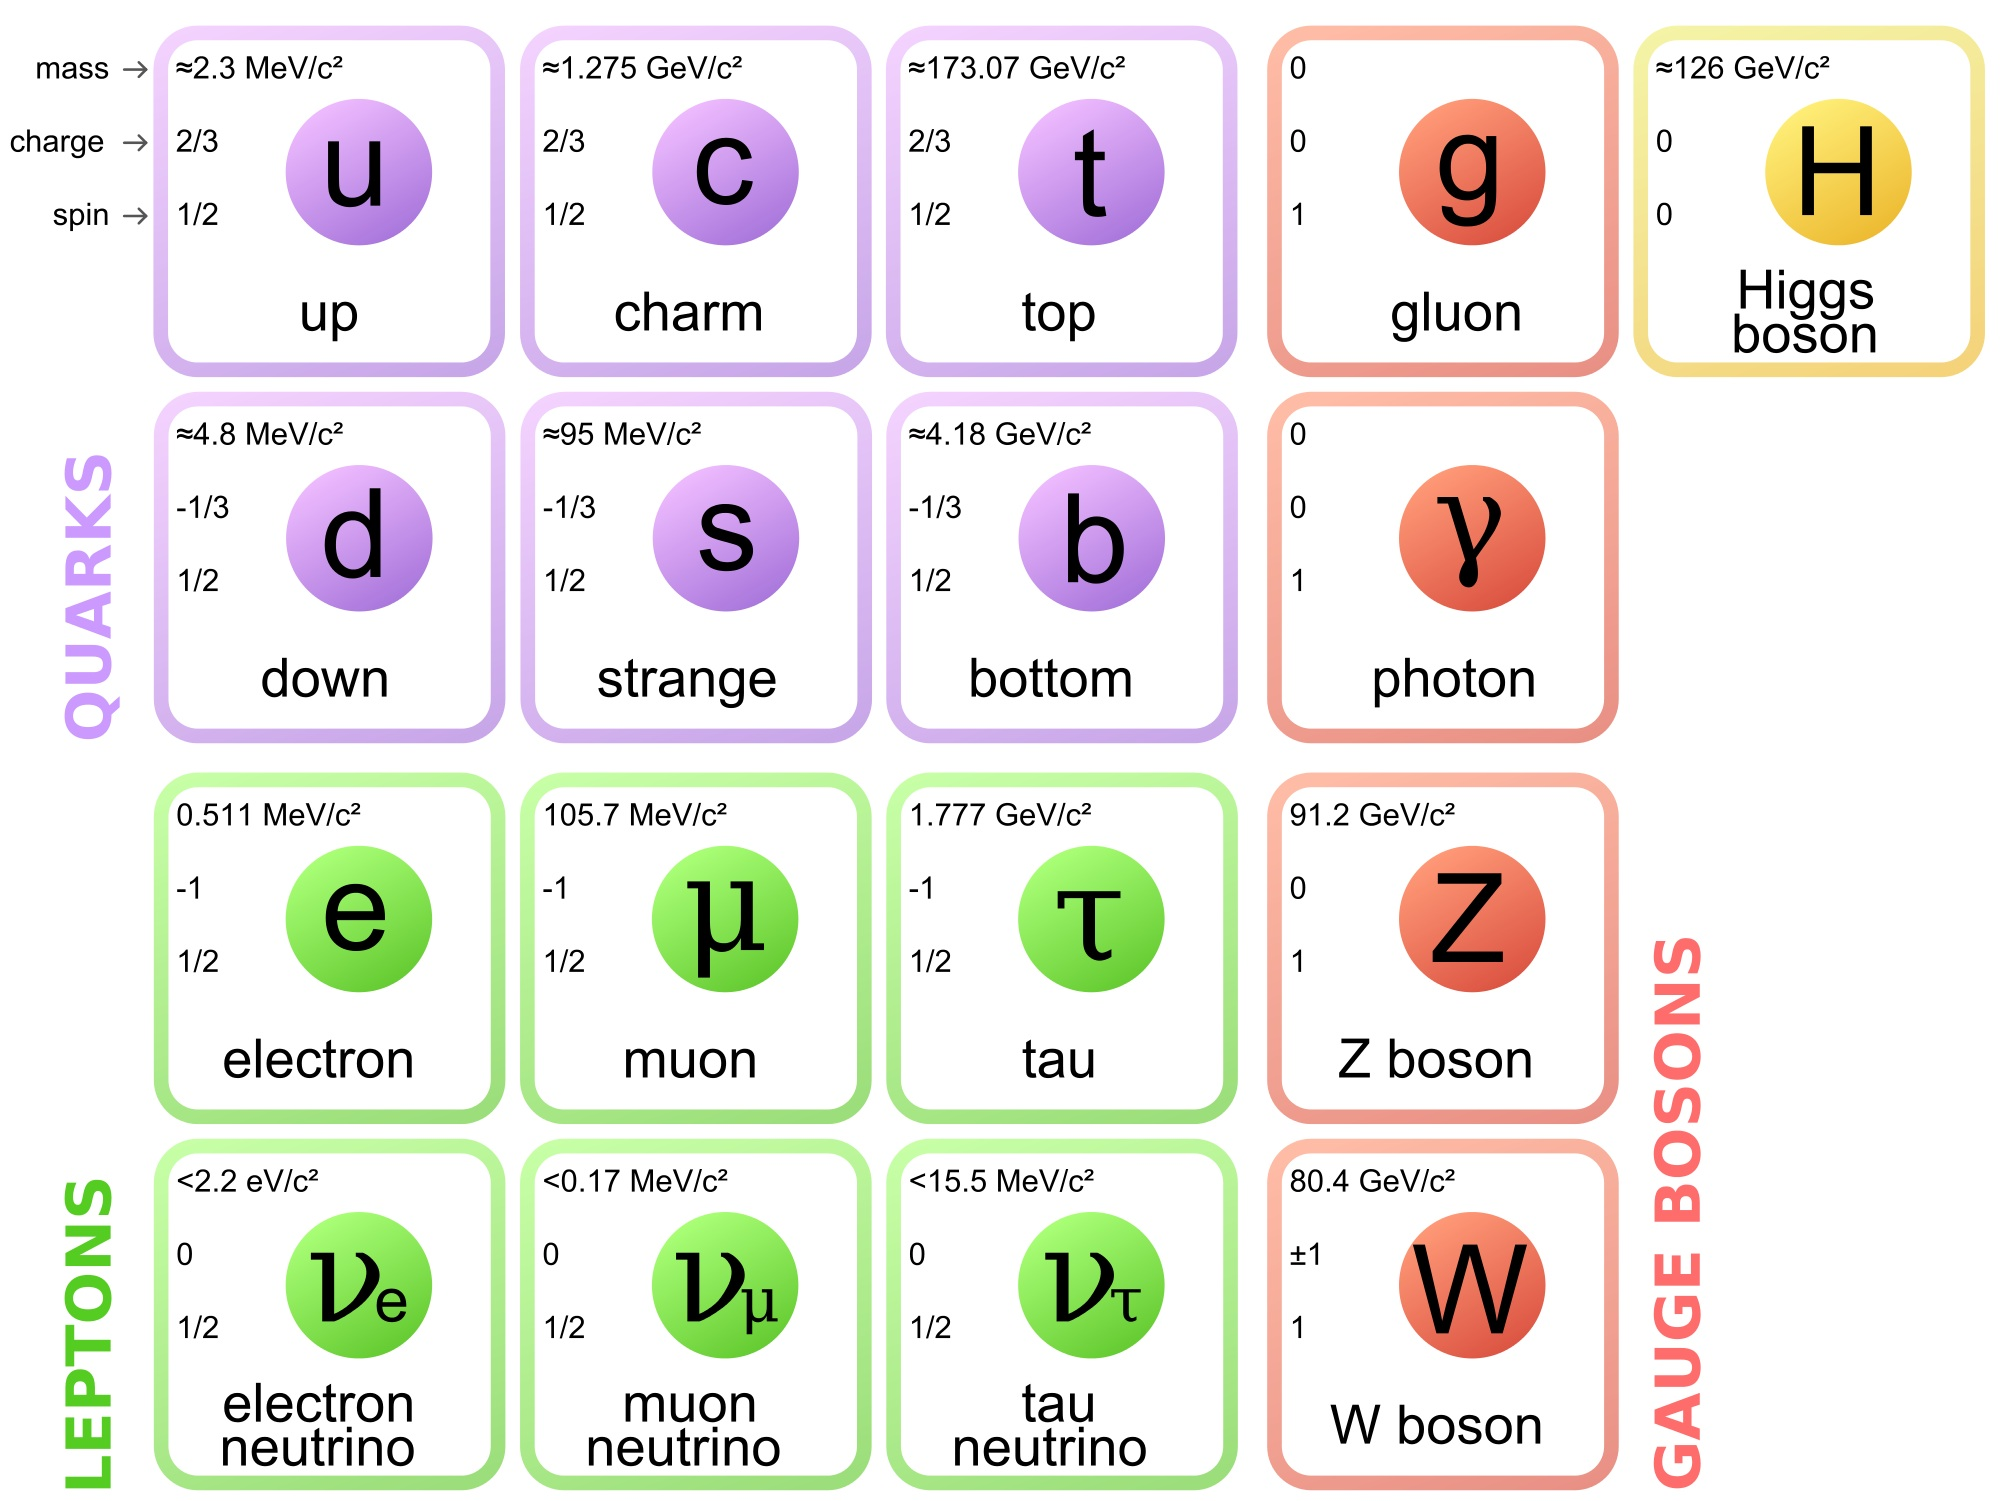
\includegraphics[width=0.8\textwidth]{Figures/standardmodel.jpg} 
 \caption{The current model of particle physics. Image courtesy of \cite{quantumdiaries}.}
\end{figure}

Similar to the electron ($e$), the muon carries a fundamental charge of $\pm$1, a total spin of 1/2, and observes the electromagnetic and weak forces. Moreover, the muon also has a corresponding neutrino: the muon neutrino ($\nu_\mu$). However, the muon (mass = 105.7 MeV/$c^2$) is about 200 times heavier than the electron (mass = 0.511 MeV/$c^2$). Indeed, sometimes it is useful to think of a muon simply as a heavy electron, but the mass implies several unique characteristics. One of these is the instability of muons, and results in muons decaying into an electron, an electron antineutrino, and a muon neutrino:
\begin{equation} \nonumber
\mu \rightarrow e+\bar{\nu}_e+\nu_\mu.\\
\end{equation}

This is quite interesting, as it means muons are a double-edged sword. On the one hand, their point-like nature means that the muon collisions are clean. That is to say, muon colliders have a great advantage over, e.g., proton colliders since protons are composed of three quarks. Each quark may have a different flavor or energy level and hence adds more variables to the analysis. Furthermore, each quark is bound and so gluon interactions must also be considered. These quarks and gluons may undergo hadronization when interacting with one another, creating a plethora of possible hadrons. Hadronization is not fully understood, and so these sprays of hadrons are typically lumped together as a single ``jet''. While there are many working models for jet analysis, none are exact. Conversely, any data from muon interactions will have relatively little noise and will not produce jets.

Clean collisions can also be achieved with linear electron colliders. Yet unlike the electron, the muon does not emit a large amount of synchrotron radiation as it is accelerated. This is because the power irradiated off a particle due to synchrotron radiation is inversely proportional to the mass of the particle to the fourth power \cite{griffithsem}:
\begin{align*}
P \propto 1/m^4.
\end{align*}
Therefore, the relative power loss due to synchrotron radiation for electrons and muons is $P_e/P_\mu\propto m_\mu ^4/m_e ^4 \approx 1.8 \text{\sc{e}}9$. Since muons lose power via synchrotron radiation at roughly one-billionth the rate of electrons, it is possible to have a circular muon accelerator. Furthermore, due to the small mass of a muon compared to a proton ($\sim$105 MeV/$c^2$ vs. $\sim$938 MeV/$c^2$), muons are easier to accelerate. This means that a muon facility can be much smaller than its proton counterpart. 

However, there is one problem with a muon accelerator. A rest frame lifetime of 2 $\mu$s requires the muons to be accelerated quickly before they decay. This is a challenge for circular colliders which require a high-intensity beam.

Overall, it appears that there are several advantages and one key disadvantage: the 2 $\mu$s mean rest frame lifetime of the muon. However, this is only a disadvantage for muon colliders. Another application, which turns the moderately short lifetime into an advantage, is a neutrino factory. This is a facility that is dedicated to the output of a neutrino beam. Muons have two primary advantages over fission reactor neutrino sources. The first is that muons decay into exactly two flavors of neutrino: electron and muon. Therefore, the initial composition of the neutrino beam would be well-defined. This is important since neutrinos can change their flavors over time. Secondly, since neutrinos have no electric charge, they cannot be manipulated via electromagnetic focusing methods. However, the beam of muons can be focused into a high-intensity beam, and the intensity of the neutrino beam will reflect this.

%-------------------------------------------------------------------------------
\Section{COSY Infinity}\label{sec:cosy}\par
COSY Infinity is a beamline simulation tool used in the design, analysis, and optimization of particle accelerators \cite{cosy}. COSY uses the transfer map approach, which evaluates the overall effect of a system on a beam of particles using differential algebra. This involves expanding an ordinary differential equation into multivariate Taylor polynomials up to arbitrary order \cite{modernMapMethods}. Each particle in this work is represented by its coordinates as a phase space vector. The form of phase space vectors used in this work is
\begin{equation}
\centering
\mathbf{Z}=
\begin{pmatrix}
x\\ y\\ l=k(t-t_0)\\a=p_x/p_0\\b=p_y/p_0\\  \delta = (E-E_0)/E_0
\end{pmatrix},
%\caption[Phase space vector $\mathbf{Z}$.]{Phase space vector $\mathbf{Z}$. Coordinates are transverse positions ($x, y$), time-of-flight in units of length ($l$), transverse angles w.r.t. the reference particle ($a, b$), and kinetic energy deviations w.r.t. the reference particle ($\delta$). The $0$ subscript in the definitions denotes the reference particle's properties.}
\label{eqn:phaseSpaceVector}
\end{equation}
where the coordinates are transverse positions ($x, y$), time-of-flight in units of length ($l$), transverse angles w.r.t. the reference particle ($a, b$), and kinetic energy deviations w.r.t. the reference particle ($\delta$). The $0$ subscript in the definitions denotes the reference particle properties.

In beam physics, phase space vectors $\mathbf{Z}$ are subject to physics processes. This subjugation can usually be represented by a differential equation. For example, a particle in an electric field is subject to the force law \cite{griffithsem}
\begin{align}\nonumber
\mathbf{F}&=Q(\mathbf{E}+\mathbf{v}\times \mathbf{B}),
\end{align}
or in terms of the momentum,
\begin{align}\nonumber
\frac{d}{dt}\mathbf{p}&=Q(\mathbf{E}+\frac{1}{m}\mathbf{p}\times \mathbf{B}).
\end{align}

Fortunately, any phase space vector $\mathbf{Z}$ in an arbitrary order ordinary differential equation (ODE) can be rewritten as a first-order ODE \cite{modernMapMethods}. For an order $n$ ODE, a first-order ODE is constructed by introducing $n-1$ new variables. This is to say that
\begin{align} \nonumber
\frac{d^n}{dt^n}\mathbf{Z}&=\mathbf{f}(\frac{d^0}{dt^0}\mathbf{Z},...,\frac{d^{n-1}}{dt^{n-1}}\mathbf{Z})
\end{align}
can be rewritten as
\begin{align} \nonumber
\frac{d}{dt} \begin{pmatrix}
		\mathbf{Z} \\ \mathbf{Z}_1 \\ \vdots \\ \mathbf{Z}_{n-1}
		\end{pmatrix}
&= 		\begin{pmatrix}
		\mathbf{Z}_1 \\ \mathbf{Z}_2 \\ \vdots \\ \mathbf{f}(\mathbf{Z},...,\mathbf{Z}_{n-1})
		\end{pmatrix}.
\end{align}
Here, $\mathbf{f}$ represents the physics processes. For the Maxwell's equations example, the equation is already first order in $a$ and $b$, with the momentum component of $\mathbf{f}$ as
\begin{align}\nonumber
\mathbf{f}(\mathbf{p})=Q(\mathbf{E}+\frac{1}{m}\mathbf{p}\times\mathbf{B})=Q(\mathbf{E}+\frac{1}{m}\left[ap_0 \hat{x} + bp_0\hat{y} + p_z \hat{z}\right]\times\mathbf{B}).
\end{align}
 Furthermore, COSY does not use time as the independent variable, but rather arc length $s$ (see Figure~\ref{fig:saxis}).

\begin{figure}[h!]
\centering
\includegraphics*[width=70mm]{./Figures/saxis}
\caption{The reference orbit. Figure courtesy of \cite{berzFullnotes}.}
\label{fig:saxis}
\end{figure}

If there exists a unique evolution of $\mathbf{Z}$ then it is possible to construct the so-called transfer map $\mathcal{M}$. Mathematically, this relationship is $\mathbf{Z}(s)=\mathcal{M}(s_0 , s)*\mathbf{Z}(s_0)$, with $*$ representing the application of the transfer map to the phase space vector $\mathbf{Z}$ at $s_0$. 

It is possible to construct a transfer map for most cases in beamline physics. This is because most beamline elements follow differential equations which yield unique solutions dependent on initial conditions (such as Maxwell's equations). If there does not exist a unique evolution of $\mathbf{Z}$ then it is not possible to construct the transfer map. Systems which produce a unique evolution of $\mathbf{Z}$ are called ``deterministic''.

An example of the relationship between the initial phase space vector, the transfer map, and the final phase space vector can be seen in Figure~\ref{fig:matrix_element_example_1}. The initial phase space occupied by the beam of particles is at the coordinate $s_0$. Physically, there exists some deterministic beamline element between $s_0$ and $s_1$. This element can be represented by the map $\mathcal{M}$, which creates a bijection for the phase space vectors $\mathbf{Z}(s_0)$ and $\mathbf{Z}(s_1)$ between the initial coordinate $s_0$ and the final coordinate $s_1$. 

Entire lattices may also be represented by a single transfer map. This is done by dividing the lattice into its base components or elements. A transfer map for each corresponding element may then be produced. For two example elements between coordinates $s_0$ and $s_2$ (see Figure~\ref{fig:matrix_element_example_2}), the composition of two maps yields another map: $\mathcal{M}(s_1 , s_2)\times \mathcal{M}(s_0 , s_1) = \mathcal{M}(s_0 , s_2)$.  Therefore, it is possible to simplify the middle part $s_1$. In this way, the transfer maps from small components build up into a single transfer map for the whole system. Computationally this is advantageous because once calculated, it is much faster to apply a single transfer map to a distribution of particles than to simulate that same distribution through many meters of individual lattice elements.

\begin{figure}[h!]
  \centering
    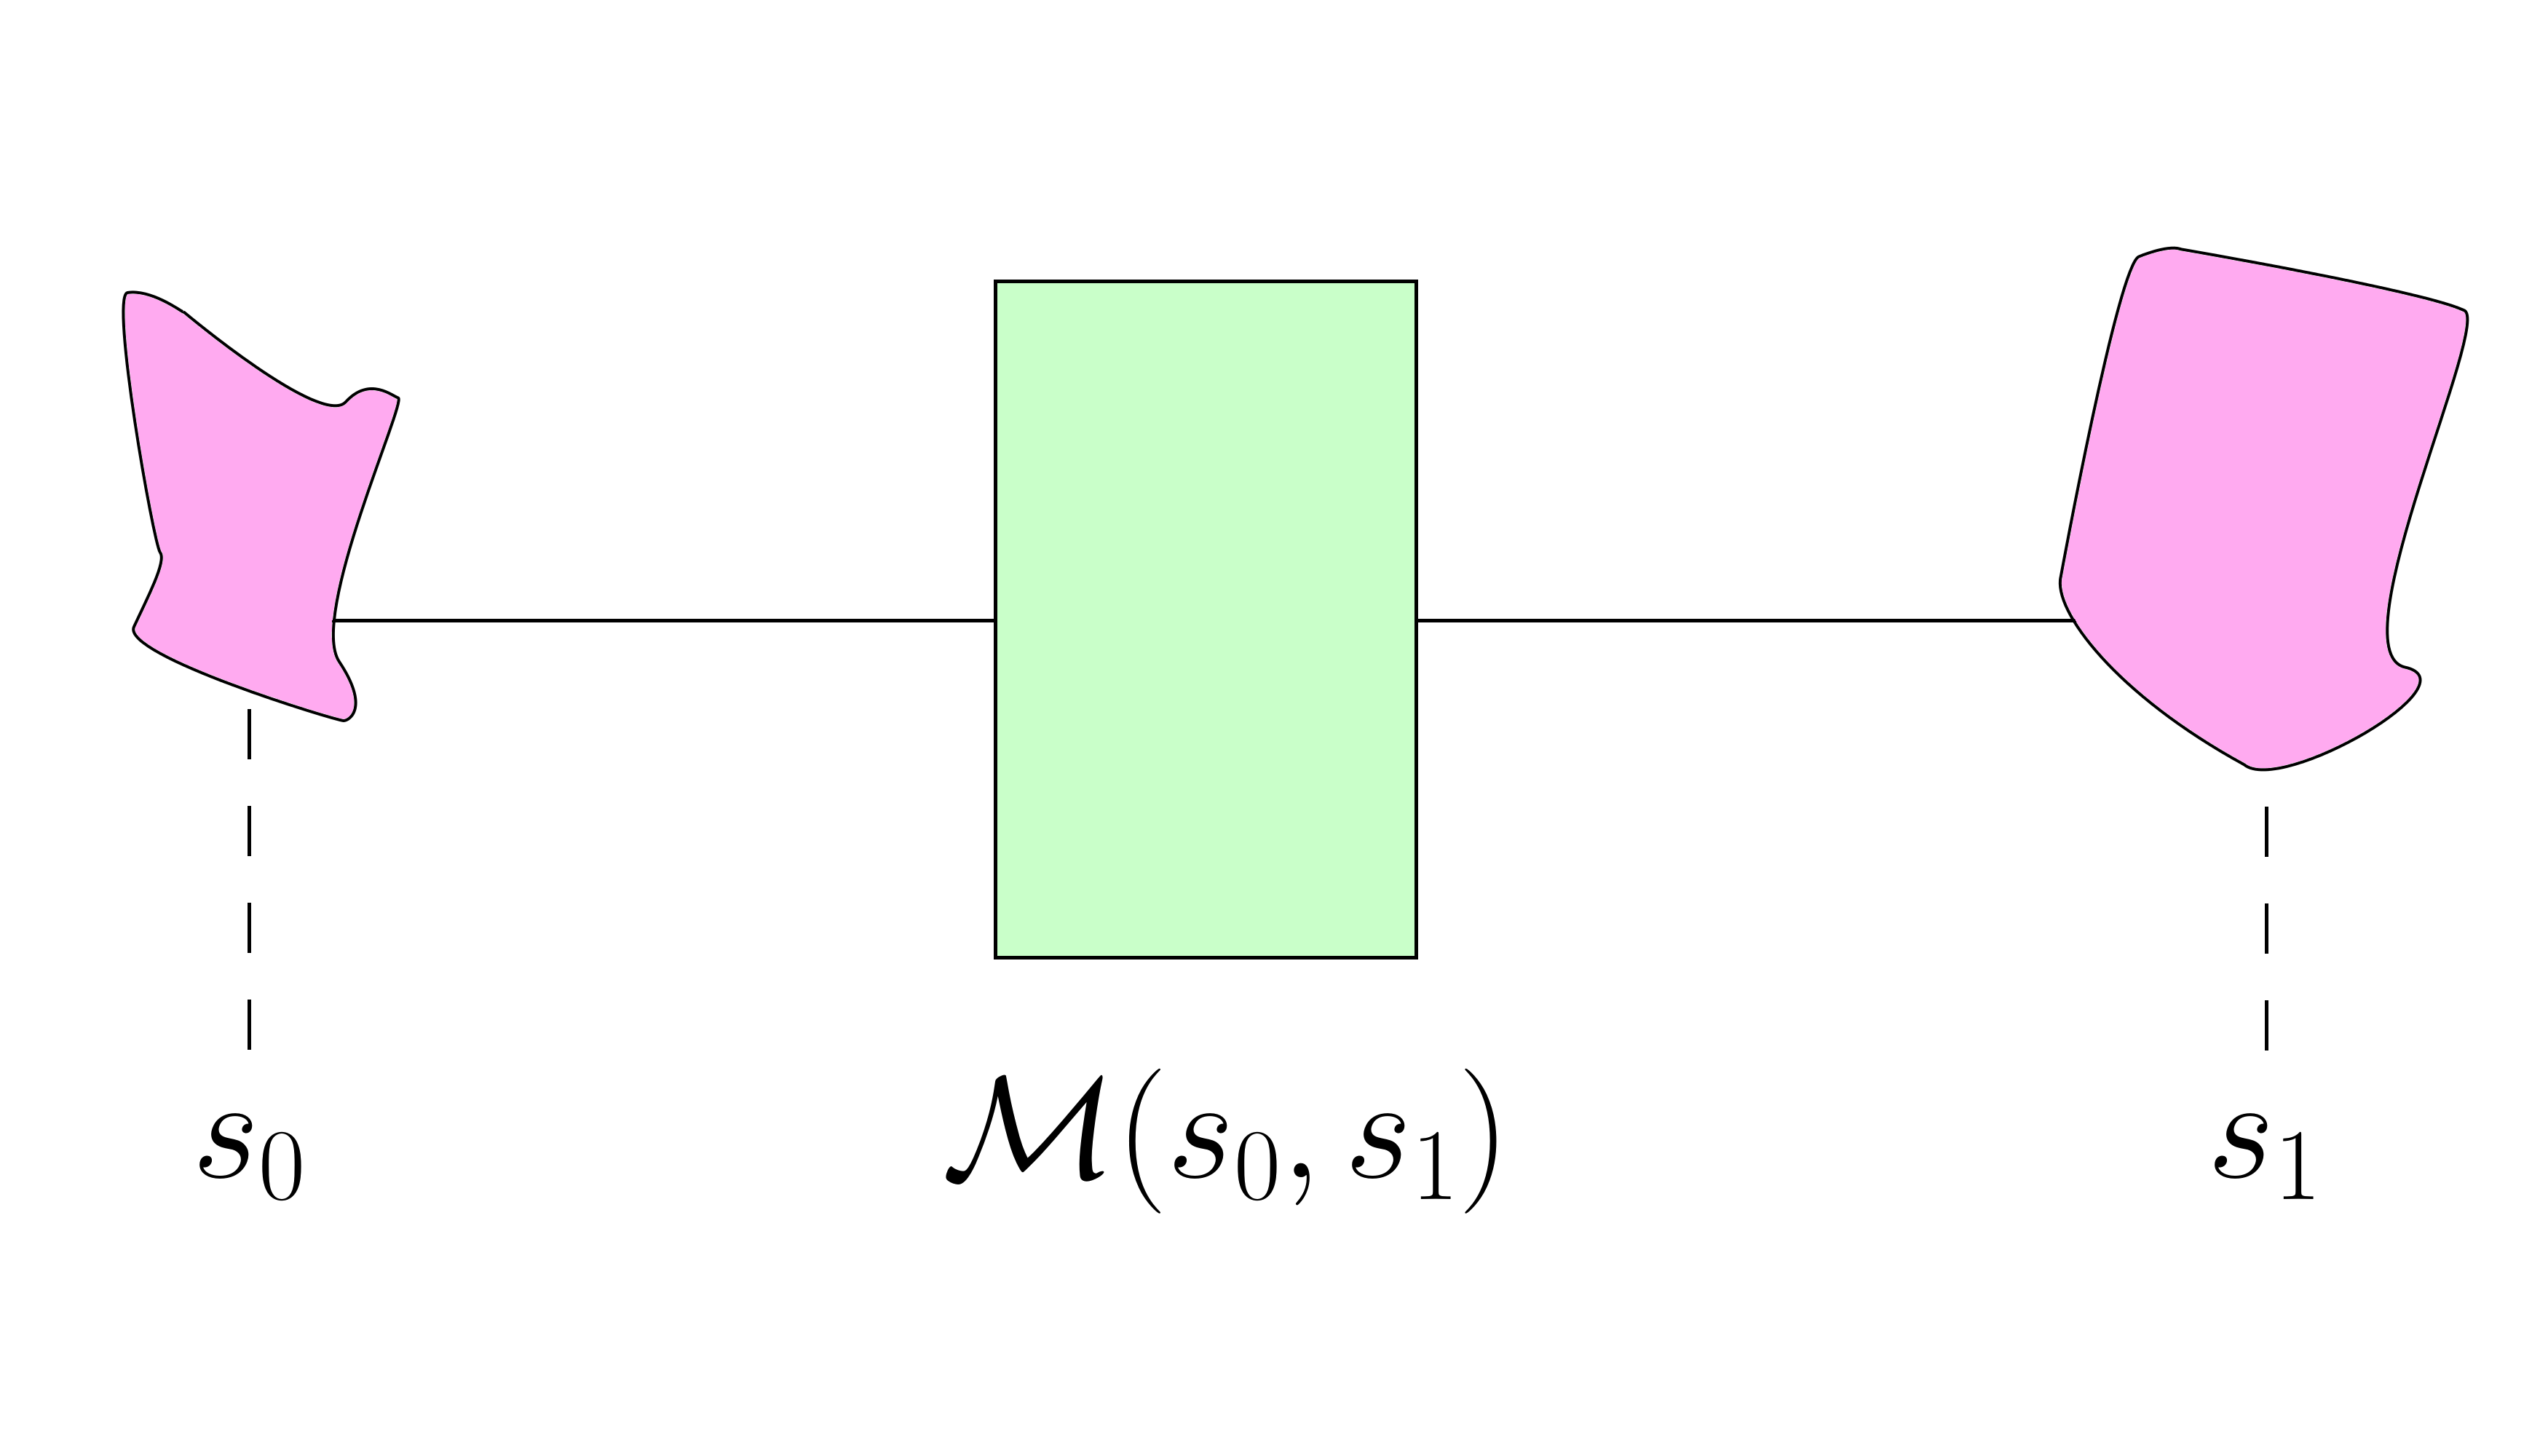
\includegraphics[width=0.75\textwidth]{Figures/matrix_element_example_1} 
  \caption{Example of some map $\mathcal{M}$ creating a bijection from $s_0$ to $s_1$.}
  \label{fig:matrix_element_example_1}
\end{figure}

\begin{figure}[h!]
  \centering
    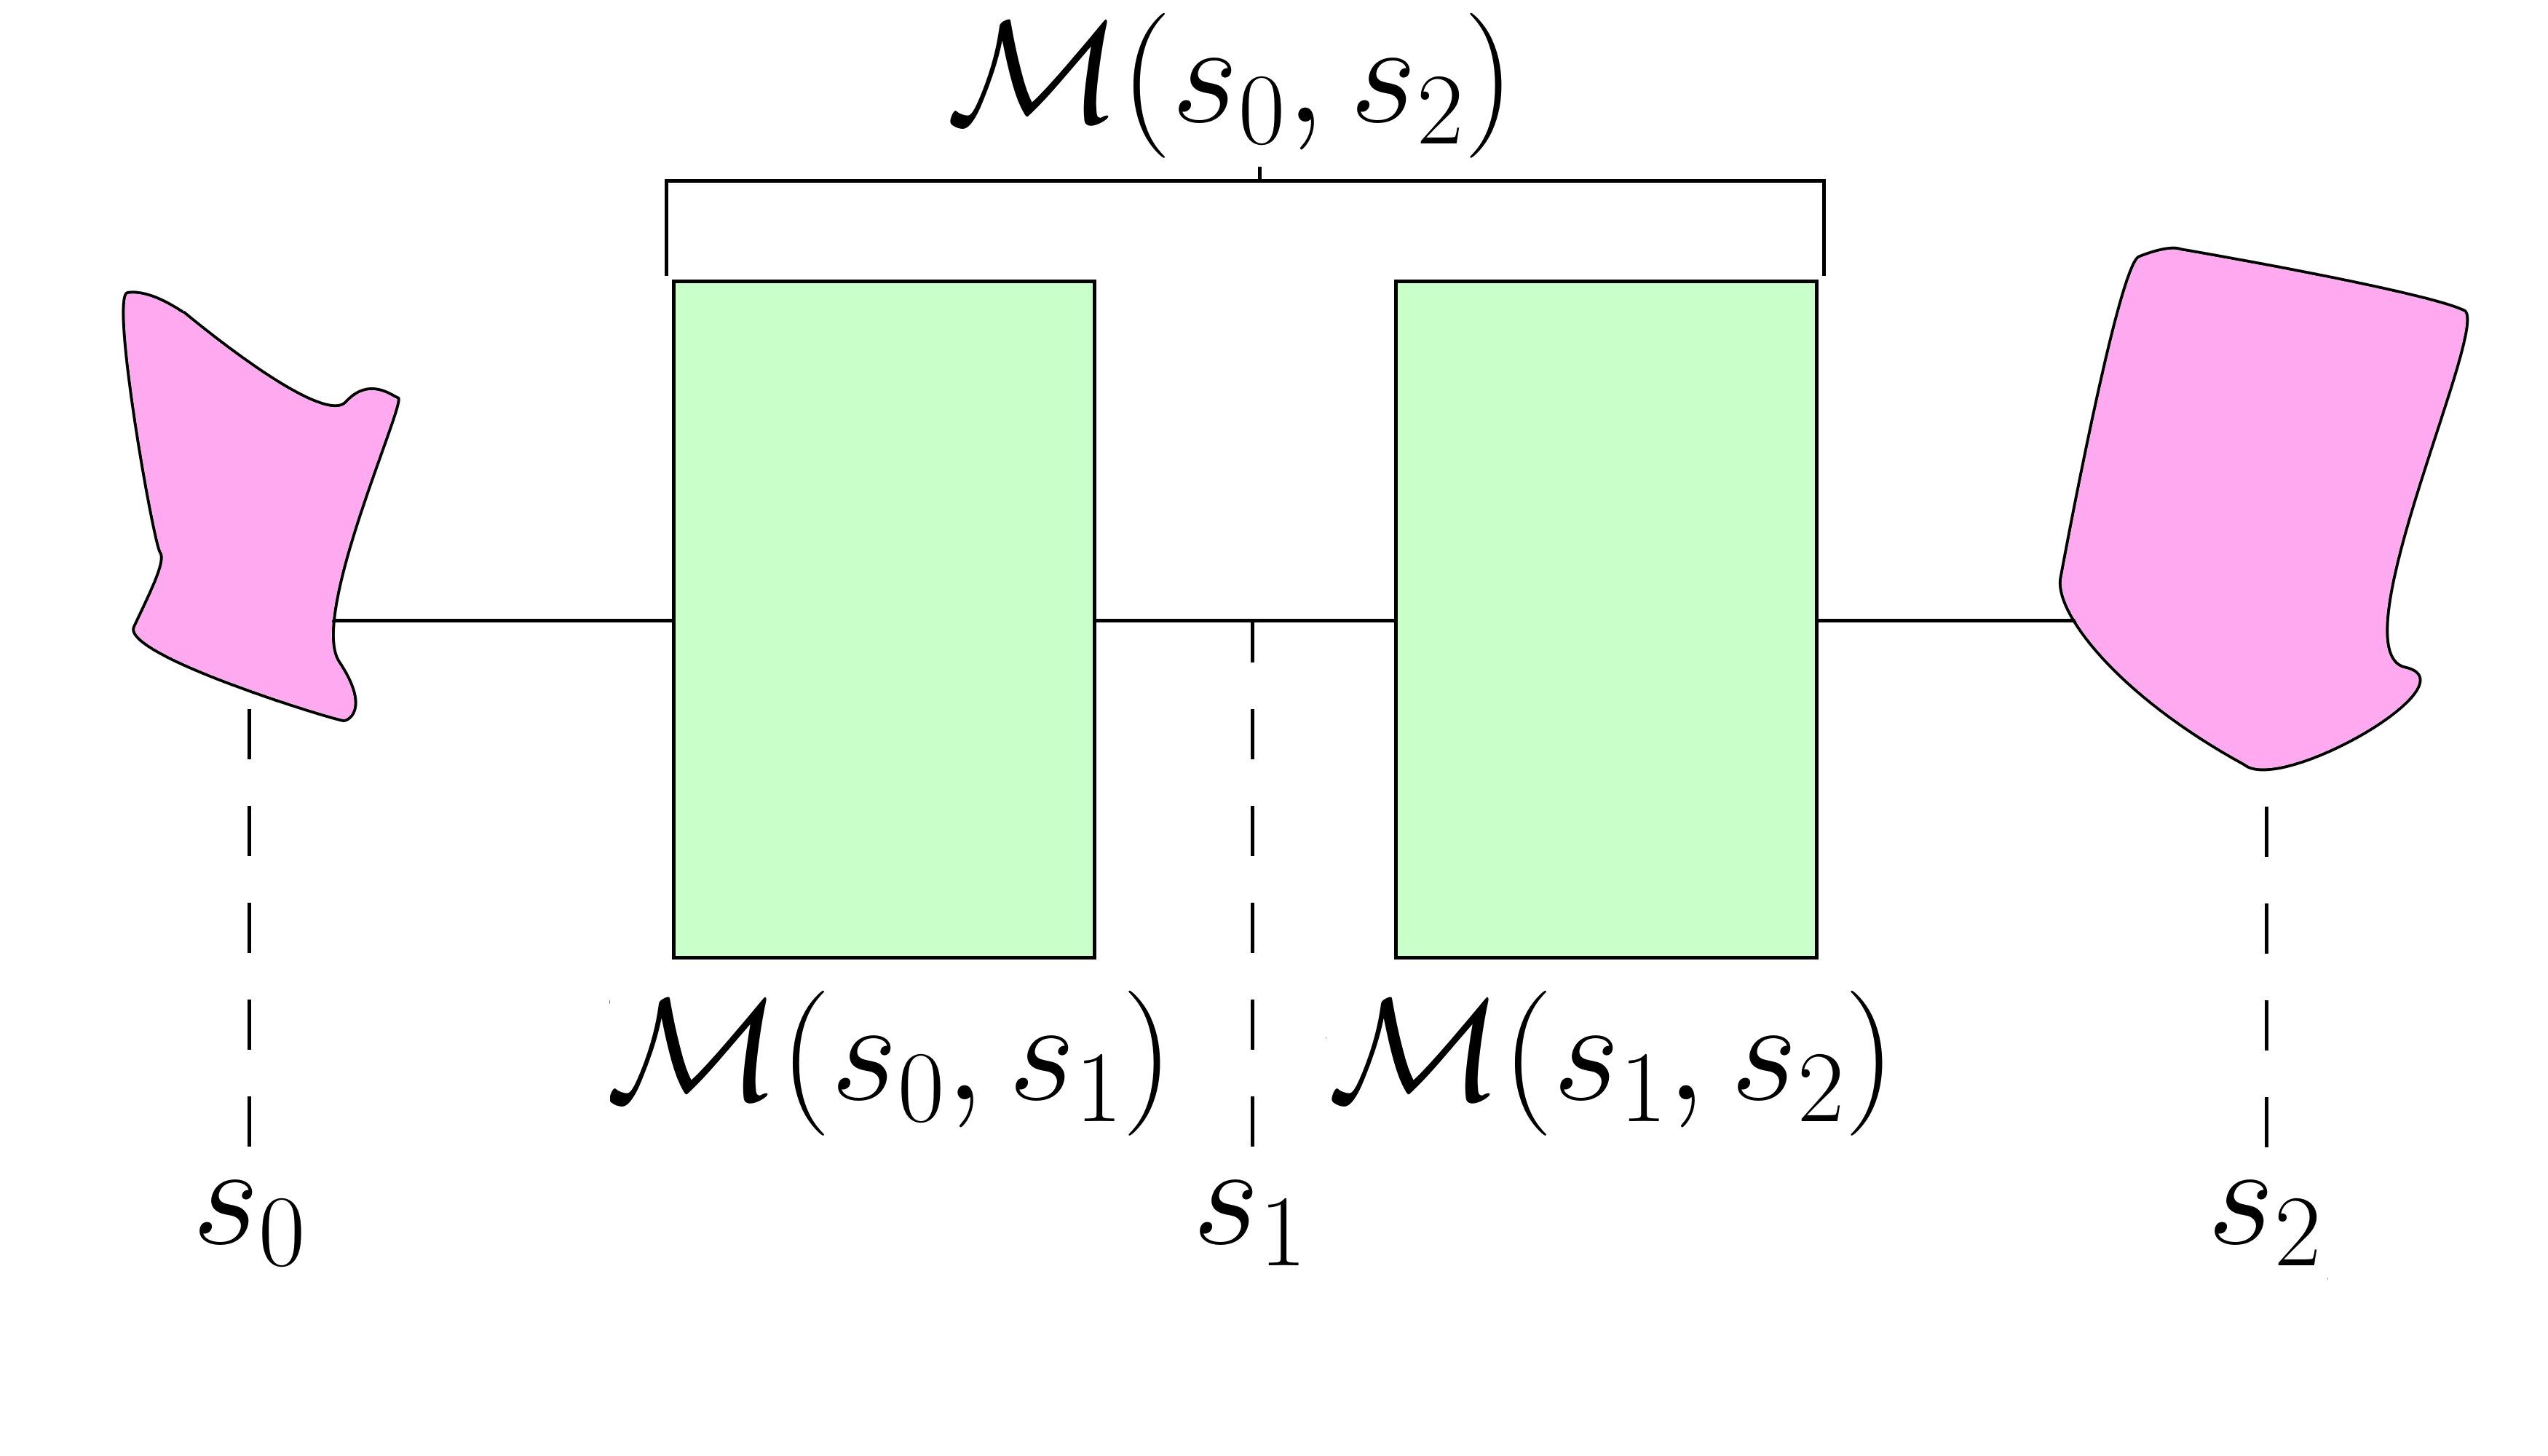
\includegraphics[width=0.75\textwidth]{Figures/matrix_element_example_2} 
  \caption{Example of two maps $\mathcal{M}(s_0,s_1)$ and $\mathcal{M}(s_1,s_2)$. These two maps may be combined together to reduce to a single map, $\mathcal{M}(s_0,s_2)$.}
  \label{fig:matrix_element_example_2}
\end{figure}

Along with the tracking of particles through a lattice, COSY also has a plethora of analysis and optimization tools, including (but not limited to) lattice aberration and correction tools, support for Twiss parameters, support for tunes and nonlinear tune shifts, built-in optimizers for lattice design, and spin tracking.

Valid elements are any beamline elements that are deterministic. Elements used in this study are magnetic multipoles (dipoles, quadrupoles, etc.), solenoidal coils, radiofrequency (RF) cavities, and drifts. Currently supported elements in COSY include but are not limited to: various magnetic and electric multipoles (with or without fringe effects), homogeneous and inhomogeneous bending elements, Wien filters, wigglers and undulators, cavities, cylindrical electromagnetic lenses, general particle optical elements, and deterministic polynomial absorbers of arbitrary order.

%-------------------------------------------------------------------------------------------------------------------------------------------------
\Section{Introduction to Matter-Dominated Lattices}\par

\Subsection{Introduction to Stochastic Effects}
This section introduces stochastic effects, or effects that are intrinsically random. These effects are in contrast to deterministic effects, which are not random and hence can be predicted exactly. 

This work concerns the interactions between a muon beam and some stationary target called the `absorber'---typically a cylinder or wedge of a material with low nuclear charge ($Z$) such as liquid hydrogen or lithium hydride. The simplest model of a beam interacting with some stationary target can be found in several textbooks \cite{nielsen,griffithsqm}, with the model from \cite{jose} illustrated in Figure~\ref{fig:scatteringmodel}.

\begin{figure}
  \centering
  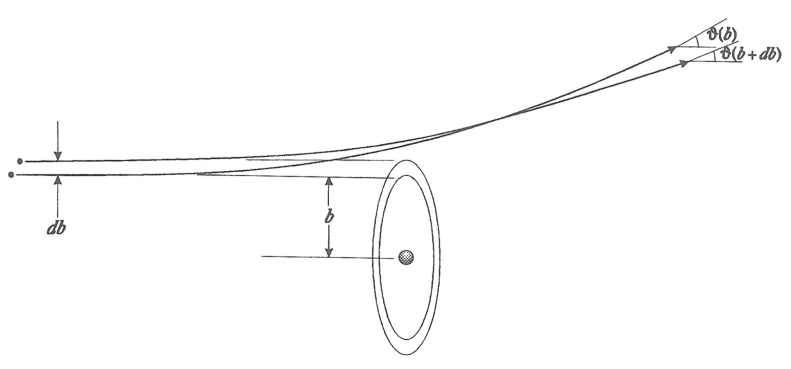
\includegraphics[width=\textwidth]{Figures/scattering_model} 

  \caption{Classical muon--target interaction model courtesy of \cite{jose}.}
  \label{fig:scatteringmodel}
\end{figure}

In this figure, $b$ is referred to as the impact parameter and is measured with respect to the particle's initial trajectory. For a beam of noninteracting particles and a perfectly stationary target, classical mechanics suggest that this is a purely deterministic problem (see, e.g., `hard-sphere scattering' in \cite{griffithsqm}); the particle with a smaller impact parameter $b$ deflects more than its neighbor with a slightly larger impact parameter of $b+db$. Since this model is entirely based on initial conditions, it would be relatively easy to implement these effects into the map methods of COSY Infinity. However, reality does not follow the model of Figure~\ref{fig:scatteringmodel}. A more accurate model is illustrated by Figure~\ref{fig:scatteringmodel2}. Here the target is still approximated as fixed, but the incident particle is now approximated as a travelling plane wave and the scattered particle is approximated as a spherical wave (at least locally).
\begin{figure}
  \centering
    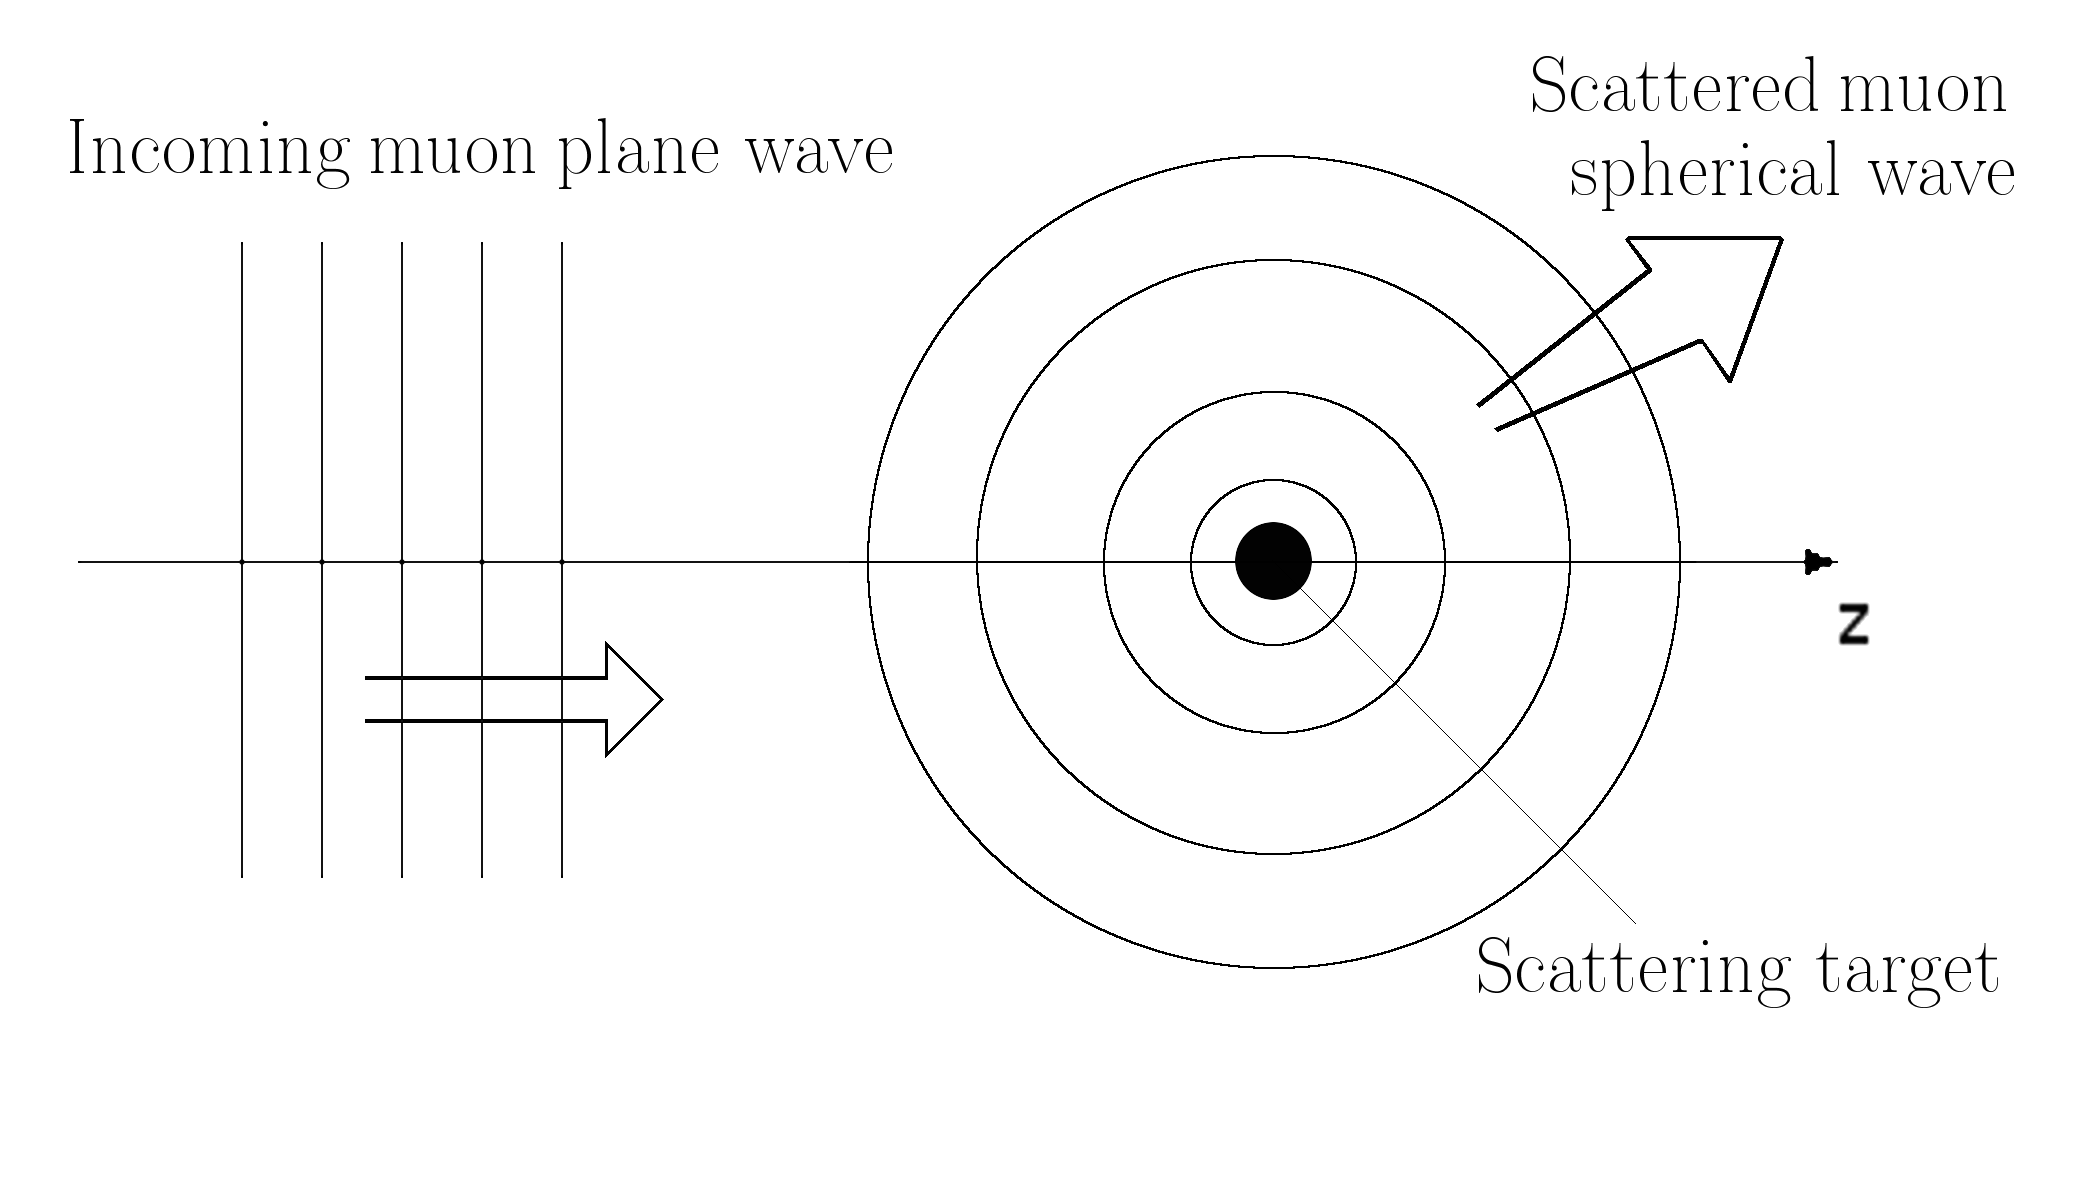
\includegraphics[width=\textwidth]{Figures/scattering_model_2} 
  \caption[Quantum muon--target interaction model.]{Quantum muon--target interaction model. The incoming particle wavefunction is represented as a plane wave and is scattered locally as a spherical wave. Image courtesy of \cite{griffithsqm}.}
  \label{fig:scatteringmodel2}
\end{figure}
It is shown later that this model predicts 
\begin{enumerate}
\item a spectrum of energy loss $\omega(\epsilon)$ which yields the probability of losing an amount of energy $\epsilon$ (see Section~\ref{sec:ICOOLStraggling}), and
\item a scattering amplitude which gives the shape of the probability distribution of scattering in a given direction $\theta$ (see Section~\ref{sec:ICOOLScattering}).
\end{enumerate}
Hence quantum theory suggests that even if two identical particles have identical initial conditions their final conditions are not the same.

\Subsection{Muon Ionization Cooling}
In Section 1.1, the primary disadvantage to the considered muon-based accelerator was the mean muon rest frame lifetime (2~$\mu$s). This is expected to be far too short of a timespan to be useful in a traditional accelerator scheme since the muons must be collected, focused, and accelerated. For the moment, observe the two proposed schematics in Figure~\ref{fig:muon_accelerator_schematic}\cite{map}. The section labeled `Proton Driver' produces protons, which will eventually yield muons. This is essential since muons do not naturally occur in great quantities at a convenient extraction point. In order to create muons, the protons strike some large target (which must be optimized to produce the highest yield), resulting in a spray of protons, muons, electrons, and pions (even shorter-lived particles consisting of a quark-antiquark pair). To further optimize this process, it is advantageous to let the pions decay into muons via $\pi^+ \rightarrow \mu^+ + \nu_\mu$. The resulting ensemble of muons is then split up into bunches. The next section in Figure~\ref{fig:muon_accelerator_schematic} is the focus of this thesis. For now, it is simply addressed as the `cooling channel' and delved into later. Cooling the beam simply means reducing the beam's phase space. Reducing the momentum of the beam results in a reduced physical size. The purpose of cooling is to increase the density of the resulting beam. This lets the beam fit into smaller magnets, which are less expensive than larger magnets. However, this increase in density also increases the luminosity of the beam in the long run. For a collider, this means more collisions; for a neutrino factory, this means more neutrino counts in the detectors (since neutrinos are neutral, there is no way to focus a neutrino beam once created). After the beam of muons is focused it is accelerated to an appropriate energy. For a neutrino factory, this is 5 GeV, and the muon and antimuon beams are allowed to decay in a storage ring. For a muon collider, the center-of-momentum energy is $\sim 126$ GeV for a Higgs factory or up to 10 TeV for high energy studies.

\begin{figure}
  \centering
    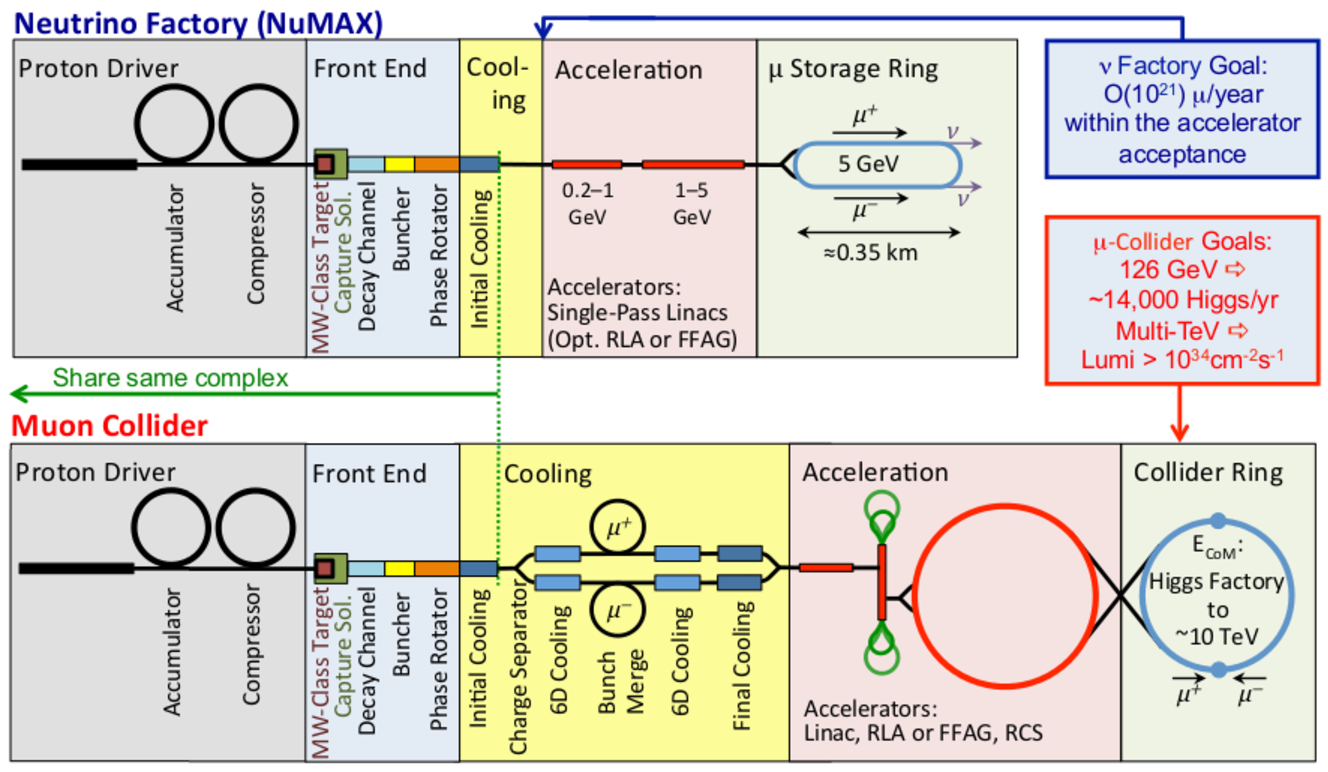
\includegraphics[width=\textwidth]{Figures/muon_accelerator_schematic} 
  \caption[Proposed muon accelerator schematics.]{Proposed muon accelerator schematics. The neutrino factory (top) is designed to produce high-intensity beams of neutrinos. The muon collider (bottom) is designed to produce high energy high-intensity beams of muons for, e.g., Higgs production. The muon collider demands more cooling and acceleration due to the higher intensity and energy threshold requirements of high energy physics. Image courtesy of \cite{map}.}
  \label{fig:muon_accelerator_schematic}
\end{figure}


The cooling channel is the crux of the entire operation for either purpose. Ionization cooling is the only cooling technique fast enough to work within the average muon lifetime. Ionization cooling requires the beam to deposit its energy in matter, thus ionizing the matter.

While the idea of ionization cooling has been around since at least 1956 \cite{oneill,lichtenberg}, it did not appear to be a viable option until roughly 1970 \cite{YuM}. It was believed that multiple scattering effects would mask any cooling benefits. Scattering is a quantum effect in which two objects are deflected when they are in close proximity at high energies, and hence is intrinsically random. This means that while the energy deposition reduced the beam's phase space, the beam would also grow in the transverse direction due to this multiple scattering.

Now, this seems to be quite the opposite of what is intended; ionization cooling potentially produces a slow, fat beam, and an effective muon beam should be narrow and fast so that the Lorentz boost keeps the muons from decaying. Fortunately, these problems can be solved simultaneously. The overall cooling scheme is presented in  Figure~\ref{fig:coolingchannel} and the vector describing the change in momentum is depicted in Figure~\ref{fig:123ionization}.
\begin{figure}
  \begin{center} 
    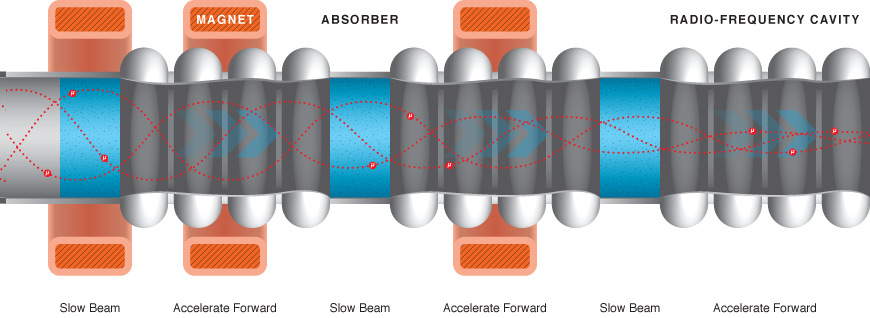
\includegraphics[width=\textwidth]{Figures/coolingchannel} 
  \caption{Cartoon of a cooling channel, courtesy of \cite{map}.}
  \label{fig:coolingchannel}
 \end{center}
\end{figure}

The key is to use a cell which contains both the ionizing material and a radio frequency cavity. To understand why this solves the problem of potentially producing a beam with a large transverse phase space, it is necessary to observe Figure~\ref{fig:123ionization}. In Figure~\ref{fig:123ionization}, the longitudinal momentum ($p_l$) is plotted against the transverse momentum ($p_t$). 
   \begin{enumerate} 
  \item{Beam deposits energy in material, reducing the momentum in all directions.}
  \item{Multiple scattering effects are observed. The transverse phase space increases (or `heats up'). By a clever choice of absorbing material (as is discussed in the next section), the growth of the transverse phase space is kept to a minimum at this stage.}
  \item{The beam is re-accelerated by the radiofrequency cavity, increasing the longitudinal momentum only. The result is a reduction in transverse momentum (i.e. blue vector compared to black vector). This solves the problem of having a large transverse phase space. Moreover, re-acceleration solves the problem of decay: after the beam loses energy, it gains that much energy again, and so the Lorentz boost stays constant on average.}
\end{enumerate}

\begin{figure}
  \centering
   \captionsetup{singlelinecheck=off}
    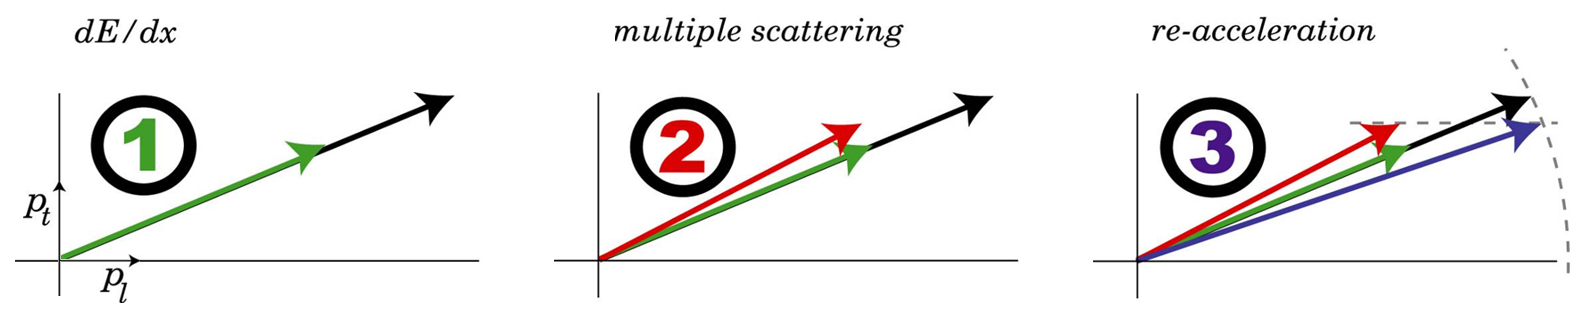
\includegraphics[width=\textwidth]{Figures/123ionization} 
  \caption{Vector diagram illustrating the principle of ionization cooling in Figure~\ref{fig:coolingchannel}. }
  \label{fig:123ionization}
\end{figure}

%-------------------------------------------------------------------------------

\Section{Emittance}\par
Emittance ($\epsilon$) is a measure of the volume of phase space occupied by the beam. It is sometimes beneficial to normalize the emittance by the relativistic factors, $\gamma$ and $\beta$. This is useful because when a beam accelerates the transverse angles decrease. This results in a  reduction of $\epsilon_x$ (where $x$ represents the general transverse direction) even though transverse phase space was not directly manipulated. However, $\epsilon_x ^N$ stays constant when a beam accelerates, and hence gives an invariant measure characterizing the beam. For the relevant transverse emittance,
%
\begin{equation}
\label{eqn:emittancedef}
%\epsilon_x^N=\beta\gamma\epsilon_x=\beta \gamma\sigma_x \sigma_\theta.
\epsilon_x^N=\beta\gamma\epsilon_x=\beta\gamma\sqrt{\left<x^2\right>\left<\theta^2\right>-\left<x\theta\right>^2}.
\end{equation}
%
Here, azimuthal symmetry is assumed, and so $x$ represents the general transverse position, and $\theta =\sin^{-1} p_x/p$ is the projection of the divergence angle of the particle trajectory onto the $x$-$z$ plane, where $z$ is the longitudinal Cartesian coordinate. 

The full derivation of the emittance in Eq. \eqref{eqn:emittancedef} can be found in Appendix~\ref{apx:emittance}. Qualitatively, if there exists no cross-dependence in $x$ and $\theta$, then the distribution should be a non-tilted ellipse. Then the emittance is proportional to the geometric mean, $\sqrt{\left<x^2\right>\left<\theta^2\right>}$. However, if there is some cross-dependence then the result is a tilted ellipse. For a sample comparison of tilted vs. non-tilted ellipses, see Figure~\ref{fig:ellipses}. Here, the emittance is outlined in red.

\begin{figure}
  \begin{center}
    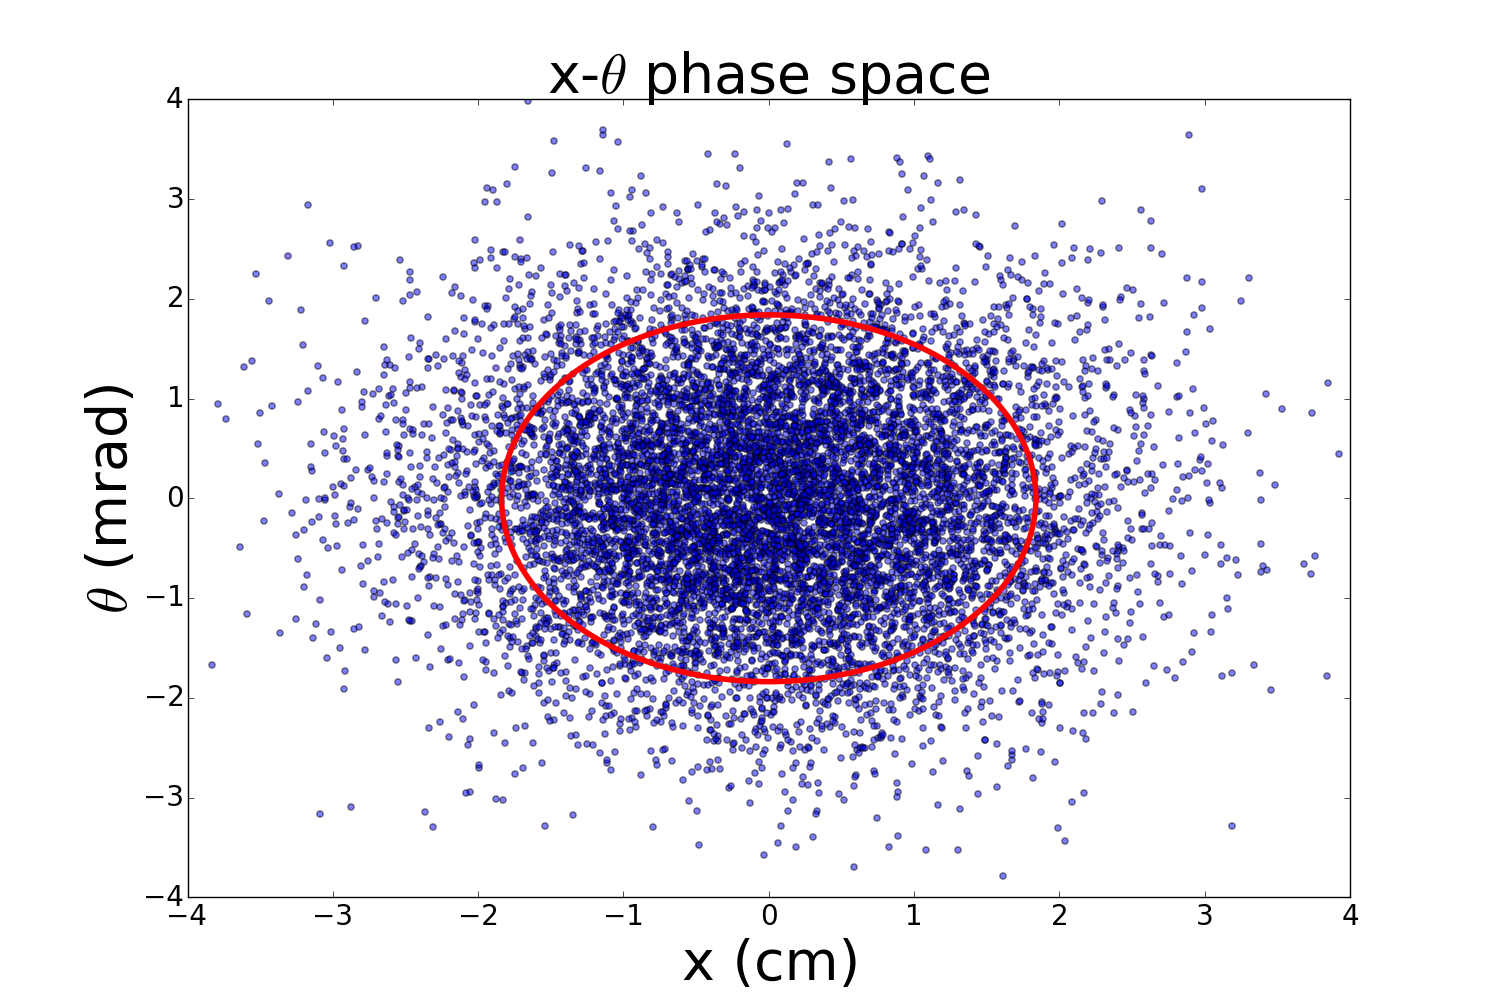
\includegraphics[width=0.49\textwidth]{Figures/ellipse0} 
    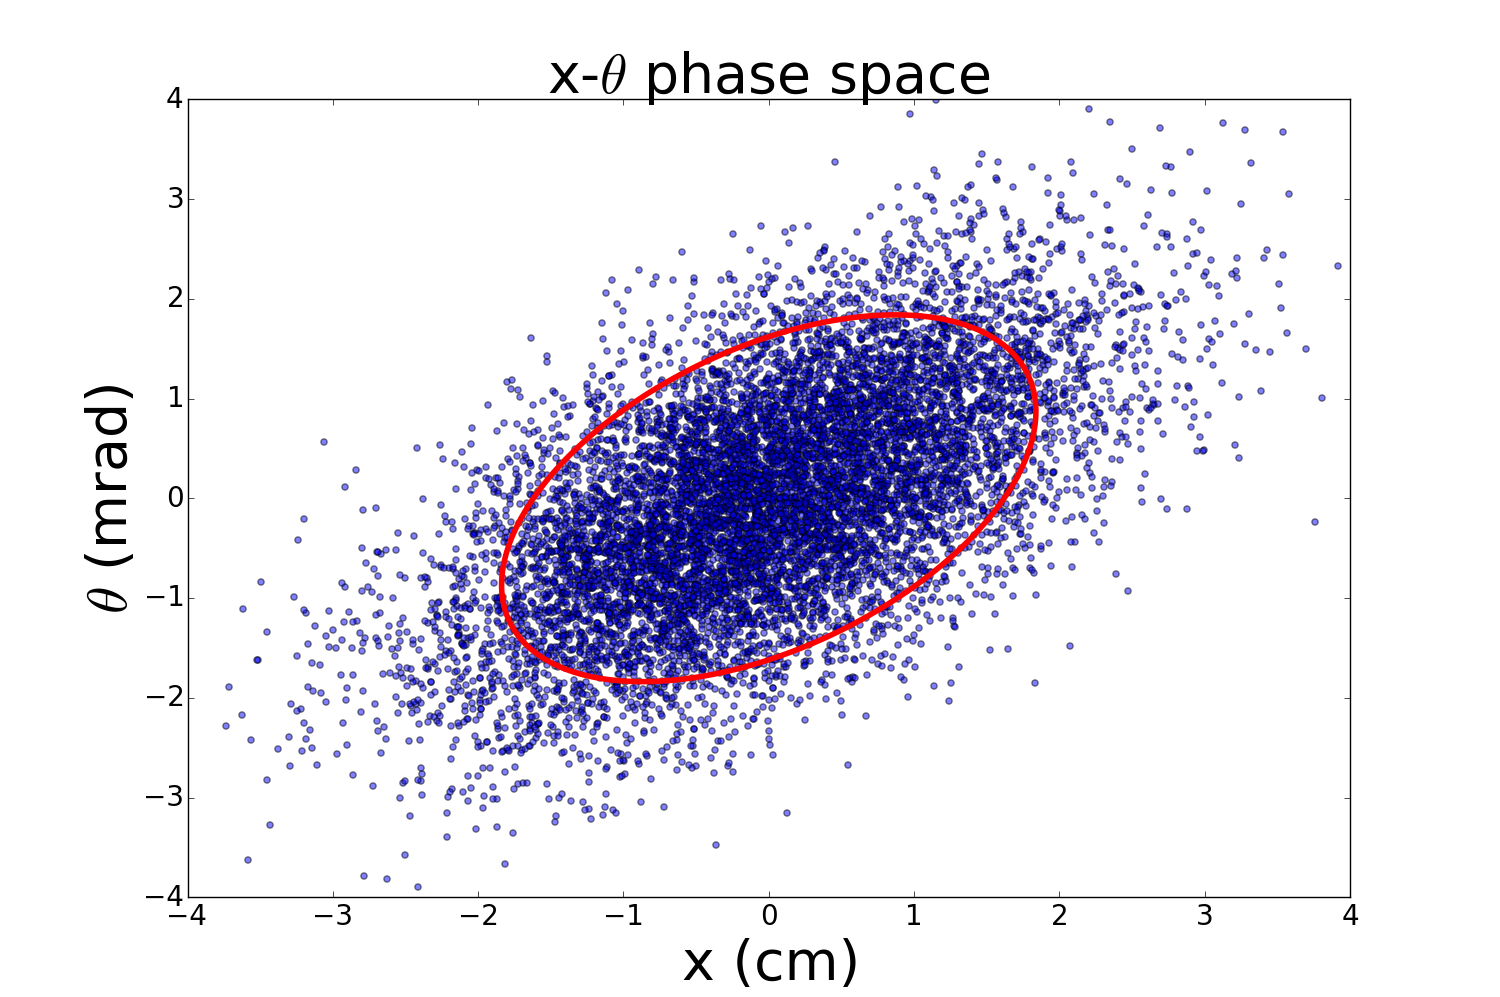
\includegraphics[width=0.49\textwidth]{Figures/ellipse1} 
  \caption[$x$-$\theta$ phase space examples.]{$x$-$\theta$ phase space examples. Left: example beam with no $x$-$\theta$ correlation ($\left<x\theta\right>=0$). Right: example beam with significant $x$-$\theta$ correlation ($\left<x\theta\right>=0.8$).}
  \label{fig:ellipses}
 \end{center}
\end{figure}

The goal is to observe the evolution of the emittance through an absorber. Taking the expression for the rate of change of normalized transverse emittance over a length $z$ from \cite{johnson},
\begin{align*}
\frac{d\epsilon^N _x}{dz}=\frac{\beta_\perp}{2}\frac{E_s^2}{\beta^3Emc^2}\frac{1}{X_0}-\frac{1}{\beta}\left| \left<\frac{dE}{dz}\right>\right| \frac{\epsilon_x^N}{E},
\end{align*}
where $\beta=v/c$ is the relativistic velocity, $\beta_\perp$ is the transverse betatron function, $E_s$ is some characteristic energy (usually 14 MeV), $E$ is the (mean) energy of the beam, $m$ is the mass of the beam species, $X_0$ is the radiation length of the absorber material, and $\left<dE/dz\right>$ is the mean energy loss of the beam through the absorber. The first term represents `heating' and the second term represents `cooling' in the transverse plane. 

Starting with the first term,
\begin{equation}
\label{eqn:emittanceheat}
\frac{d\epsilon_x^N}{dz}(heat) = \frac{\beta_\perp}{2}\frac{E_s^2}{\beta^3Emc^2}\frac{1}{X_0}.
\end{equation}
Now it is clearer why this is referred to as the heating term. Since the derivative of emittance is positive, this part represents emittance growth. Moreover, to reduce this growth it is necessary to have highly energetic particles through a material with a large radiation length (typically $X_0 \propto 1/Z$ (nuclear charge)).

\iffalse




Now it is possible to derive the effect of cooling absorbers on emittance as it pertains to muon ionization cooling. Closely following \cite{Fernow}, since the goal is to observe the evolution of the emittance through an absorber, Eq. \eqref{eqn:emittancedef} is differentiated by $z$:
%
\begin{equation}
\label{eqn:emittance1}
\frac{d\epsilon_x^N}{dz}=\epsilon_x \frac{d(\beta\gamma)}{dz}+\beta\gamma\frac{d\epsilon_x}{dz},
\end{equation}
%
It will soon be shown that the first term represents `cooling' and the second term represents `heating' in the transverse plane. As such, the first term is denoted as $d\epsilon_x^N/dz (cool)$ and the second term is denoted as $d\epsilon_x^N/dz (heat)$. Starting with the second term,
%
\begin{equation} \nonumber
\frac{d\epsilon_x^N}{dz}(heat)=\beta\gamma\frac{d\epsilon_x}{dz}.
\end{equation}
%

It can be assumed that the cooling is taking place near the beam waist (that is, the part of the trajectory where the beam spread is smallest). For this case, it is a reasonable approximation that the transverse phase space has little $x$--$\theta$ cross-dependence, and so the $\left<x\theta\right>$ term may be neglected. Furthermore, with strong focusing it is possible to neglect the overall change in transverse position of the beam \cite{Fernow} (that is, $d/dz \left<x^2\right>=0$). Using these two approximations, the only derivative in the heating term is that of $\left<\theta^2\right>$:
\begin{equation} \nonumber
\frac{d\epsilon_x^N}{dz}(heat)\approx\beta\gamma\frac{d}{dz}\sqrt{\left<x^2\right>\left<\theta^2\right>}\approx \frac{\beta\gamma}{2\epsilon_x}\left<x^2\right>\frac{d}{dz}\left<\theta^2\right>.
\end{equation}

From betatron focusing theory, at the beam waist $\left<x^2\right>$ may be rewritten as $\beta_\perp \epsilon_x$, where $\beta_\perp$ is the transverse betatron function. Moreover, using \cite{highland} $\left<\theta^2\right>$ can be written as $h(z)/\beta^2E$. Here, $h(z)$ is the Highland $z$-dependence, the form of which many theories disagree. However, the first order term of $h(z)$ is generally not model-dependent, and so this becomes
\begin{equation} \nonumber
\left<\theta^2\right>\approx\frac{E_s}{\beta^2 E}\sqrt{\frac{z}{X_0}},
\end{equation}
where $E_s$ is some characteristic energy ($\approx14$ MeV) and $X_0$ is the radiation length of the given material. Then
\begin{equation} \nonumber
\frac{d\epsilon_x^N}{dz}(heat)\approx\beta\gamma\frac{\beta_\perp}{2}\frac{d}{dz}\left(\frac{E_s}{\beta^2 E}\sqrt{\frac{z}{X_0}}\right),
\end{equation}

\begin{equation}
\label{eqn:emittanceheat}
\frac{d\epsilon_x^N}{dz}(heat)\approx\frac{\beta_\perp}{2}\frac{E_s^2}{\beta^3Emc^2}\frac{1}{X_0}.
\end{equation}

Now it is clearer why this is referred to as the heating term. Since the derivative of emittance is positive, this part represents emittance growth. Moreover, to reduce this growth it is necessary to have highly energetic particles through a material with a large radiation length (typically $X_0 \propto 1/Z$ (nuclear charge)).

Observe the cooling term of Eq. \eqref{eqn:emittance1}:
\begin{equation} \nonumber
\frac{d\epsilon_x^N}{dz}(cool)=\epsilon_x\frac{d(\beta\gamma)}{dz}=\epsilon_x\cdot(\beta\frac{d\gamma}{dz}+\gamma\frac{d\beta}{dz}).
\end{equation}
First,
\begin{equation} \nonumber
\frac{d\beta}{dz}=\frac{d}{dz}(1-\gamma^{-2})^{\frac{1}{2}}=\frac{1}{\beta\gamma^3}\frac{d\gamma}{dz},
\end{equation}
and then,
\begin{equation} \nonumber
\frac{d\gamma}{dz}=\frac{\gamma}{E}\frac{dE}{dz},
\end{equation}
with $E$ as the total energy of the muon beam. Finally,
\begin{equation} \nonumber
\frac{d\epsilon_x^N}{dz}(cool)=\epsilon_x\cdot(\beta\frac{d\gamma}{dz}+\gamma\frac{1}{\beta\gamma^3}\frac{d\gamma}{dz})=\epsilon_x\cdot\frac{d\gamma}{dz}\beta(1+\frac{1}{\beta^2\gamma^2}) \vspace*{12pt}
\frac{d\epsilon_x^N}{dz}(cool)=\epsilon_x\frac{dE}{dz}\frac{\gamma}{E\beta}.
\end{equation}
Normalizing the emittance by first multiplying and then dividing by $\beta\gamma$ results in
\begin{equation} \nonumber
\frac{d\epsilon_x^N}{dz}(cool)=\frac{1}{\beta}\frac{dE}{dz}\frac{\epsilon_x^N}{E}
\end{equation}
However, there are two corrections which should be observed. First, even for a perfect monoenergetic beam energy loss is stochastic, not deterministic. Two muons with identical initial conditions will likely lose different amounts of energy as they pass through the same medium. Since emittance is a collective effect, is it more appropriate to talk about an average energy loss, which turns $\frac{dE}{dz}$ into $\left<\frac{dE}{dz}\right>$. The second observation is with regard to sign convention. Typically, one refers to energy loss as a positive quantity (e.g. the beam lost 10 MeV from point A to point B), even though it is clear that $\frac{dE}{dz}$ is negative. For this reason, the energy loss term must again be changed from $\left<\frac{dE}{dz}\right>$ to  $-\left|\left<\frac{dE}{dz}\right>\right|$. This leaves the full cooling term as






\fi

Now for the second term:

\begin{equation}
\label{eqn:emittancecool}
\frac{d\epsilon_x^N}{dz}(cool)=-\frac{1}{\beta}\left| \left<\frac{dE}{dz}\right>\right| \frac{\epsilon_x^N}{E}.
\end{equation}
Similarly to the heating term, it is now understandable why this is referred to as the cooling term. The rate of change of the normalized transverse emittance is negative, and so the transverse phase space shrinks. However, at this point Eq. \eqref{eqn:emittancecool} does not explain precisely how the rate changes, and so is purely conceptual. The shape of the cooling term is determined by the average energy loss, $\left|\left<\frac{dE}{dz}\right>\right|$. However, usually it is not $\left|\left<\frac{dE}{dz}\right>\right|$ that is measured, but rather the stopping power $S(E)=-\frac{1}{\rho}\left<\frac{dE}{dx}\right>$, typically in units of MeV$\cdot$cm$^2$/g. A good example of a stopping power curve can be seen in Figure~\ref{fig:bethecurve} \cite{PDG}. For this example, there are several effects noted in Figure~\ref{fig:bethecurve}. One may be tempted to think that based on \ref{eqn:emittancecool} the most cooling should occur in the Anderson-Ziegler regime at $\beta\gamma\sim0.01$. This may seem correct since there is a $1/E$ dependence in Eq. \eqref{eqn:emittancecool}, and so the high energy part of the curve is not advantageous. Indeed, for $\rho= 8.92$ g/cm$^3$ it is easy to see that at $\beta\gamma=0.01$ 
\begin{align*}
\frac{d\epsilon_x^N}{dz}(cool)\approx-900 \text{ cm}^{-1} \cdot \epsilon_x^N.
\end{align*}

However, the correct strategy is just the opposite---one should endeavor to build a cooling cell with the minimum ionization point in mind (in the Bethe regime, where $\beta\gamma\sim2$). At the peak ($\beta\gamma\sim0.01$), the muon beam slows down quite a bit through a single cooling cell and one is at risk of losing the beam to decay. Moreover, Figure~\ref{fig:bethecurve} only depicts the stopping power, not the actual energy loss that individual particles experience. The individual energy loss is a stochastic effect, and the distribution of energy losses broadens with decreasing beam energy. This means that for lower energies, there are more particles that stop completely. 
\iffalse



Further, with a higher beam energy the stochastic energy loss profile is more sharply peaked, and so there are fewer decays and more particles that are in the RF stability region. (Remember, the longitudinal emittance is observed by the RF cavities, as seen in Figure~\ref{fig:coolingchannel}. The longitudinal emittance increases with energy loss according to \cite{Fernow}.) 



\fi
Finally, Eq. \eqref{eqn:emittanceheat} suggests that higher energies are better since they reduce the heating term. For these reasons, it is apparent that a muon cooling cell should be made of low-$Z$ materials such as liquid hydrogen or lithium hydride and operate anywhere between 100 MeV/$c$ and 400 MeV$/c$.

\begin{figure}
  \centering
    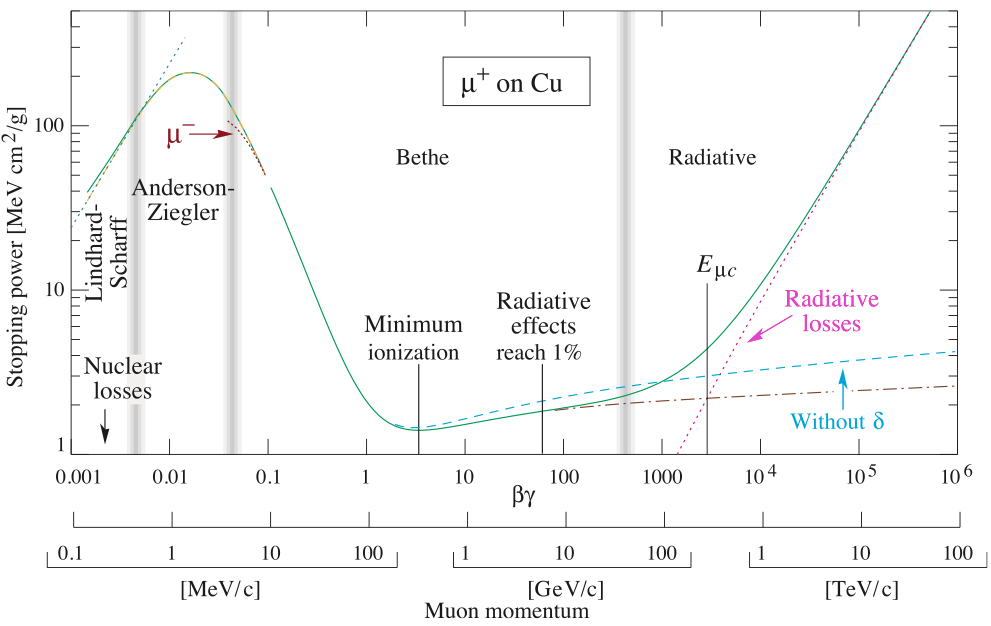
\includegraphics[width=\textwidth]{Figures/bethecurve} 
  \caption{Stopping power curve for antimuons on copper, courtesy of \cite{PDG}. }
  \label{fig:bethecurve}
\end{figure}

When particles impinge upon a fixed target, they lose some of their energy. For massive particles like muons, there are a number of major effects that contribute. However, it is important to note that in the muon cooling regime only ionization contributes significantly to the energy loss. To see this, take for an example the relatively heavy element of iron\footnote{While iron would not likely be used as an absorber material, it serves as an exaggerated example due to its $Z$ value of 9.}. In Table~\ref{tbl:elossfe}, the energy loss contributions of these four effects can be seen. However, the non-ionization effects only start to contribute at an initial beam kinetic energy of 1.40 GeV---far outside of the muon cooling regime.

\iffalse % Recreate figure as a table
\begin{figure}
  \centering
    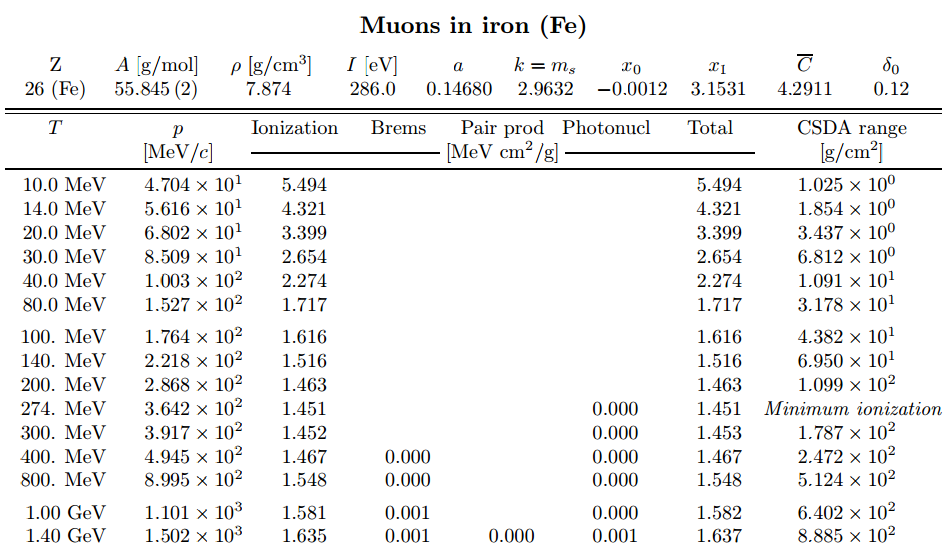
\includegraphics[width=\textwidth]{Figures/E_loss_Fe} 
  \caption{Energy loss table for muons in iron. Table courtesy of \cite{PDGTables}.}
  \label{fig:elossfe}
\end{figure}
\fi

\begin{table}
\caption*{\textbf{Muons in Iron (Fe)}}
\begin{tabularx}{\textwidth}{cccccccc}
\hline \hline
$T$ & $p$ & Ionization & Brems & Pair prod & Photonucl & Total & CSDA range\vspace{-12pt}\\
MeV & MeV/$c$ & \multicolumn{2}{c}{\sout{\hspace{3cm}}} & MeV cm$^2$/g & \multicolumn{2}{c}{\sout{\hspace{3cm}}} & g/cm$^2$\\ \hline
10 & 47.04 & 5.494 & &&& 5.494 & 1.025\vspace{-12pt}\\
14 & 56.16 & 4.321 & & & & 4.321 & 1.854\vspace{-12pt}\\
20 & 68.02 & 3.399 &  &   &  			& 3.399 & 3.437 \vspace{-12pt}\\
30 & 85.09 & 2.654 &  &  &  			& 2.654 & 6.812 \vspace{-12pt}\\
40 & 100.3 & 2.274 &  &  &  			& 2.274 & 10.91 \vspace{-12pt}\\
80 & 152.7 & 1.717 &  &  &  			& 1.717 & 31.78 \vspace{-12pt}\\
100 & 176.4 & 1.616 & &   &  			& 1.616 & 43.82 \vspace{-12pt}\\
140 & 221.8 & 1.516 & &   &  			& 1.516 & 69.50 \vspace{-12pt}\\
200 & 286.8 & 1.463 & &   &  			& 1.463 & 109.9 \vspace{-12pt}\\
274 & 364.2 & 1.451 & &   &  			& 1.451 & $Min.\, ionization$ \vspace{-12pt}\\
300 & 391.7 & 1.452 & &   &  			& 1.453 & 178.7 \vspace{-12pt}\\
400 & 494.5 & 1.467 & &   &  			& 1.467 & 247.2 \vspace{-12pt}\\
800 & 899.5 & 1.548 & &   &  			& 1.548 & 512.4 \vspace{-12pt}\\
1000 & 1101 & 1.581  & 0.001 & &  		& 1.582 & 640.2 \vspace{-12pt}\\
1400 & 1502 & 1.635  & 0.001 & & 0.001 	& 1.637 & 888.5\\
\hline
\end{tabularx}
\caption[Energy loss table for muons in iron. Table courtesy of \cite{PDGTables}.]{Energy loss table for muons in iron. Table courtesy of \cite{PDGTables}. The first two columns show $T$, the kinetic energy of the beam, and $p$, the corresponding momentum of the beam. The next four columns show the various contributions to energy loss, with column 7 giving the total energy loss. Finally, column 8 shows the range of muons through the material calulated by the continuous slowing down approximation.}
\label{tbl:elossfe}
\end{table}

This is a good example because all of the cooling materials currently being considered have less muon stopping power than iron. This means that iron represents the maximum contribution of non-ionization energy loss per initial beam energy; that is, the non-ionization effects begin to emerge at much higher energies for lighter materials such as liquid hydrogen. Note that Figure~\ref{fig:bethecurve} may also be useful when discussing this subject, as the minimum ionization regime is explicitly characterized.

%-------------------------------------------------------------------------------
\Section{Looking Forward}\par

In short, this work uses basic principles to successfully implement muon ionization cooling simulation tools into COSY Infinity. The algorithms which have been implemented are derived from first or second principles as can seen from other codes in Chapter \ref{chp:other_codes} and novelly in Chapter \ref{chp:cosy}. Furthermore, these algorithms are augmented by fitting the results to experimental data and benchmarking against external sources. The results of benchmarking and validation are discussed in Chapter \ref{chp:results}. Here, it is shown that the new routines in COSY produce robust, accurate, and fast simulations.